\maketitle

Due: Wednesday, February 7 at 11:59 pm.

\section{Practice problems -- do not submit}
\subsection*{9.5. Lines and planes in space}
\begin{practice}p.780 \#44\end{practice}
\begin{pracsol}
  Substitute values for $x,y,z$ as determined by the parametric equations into the equation for the plane to obtain
  \[(4-t)+(2t+6)-3(2t+5)=5,\]
  or
  \[-5t=10,\]
  or $t=-2$. The line meets the plane when $t=-2$. Now substitute $t=-2$ into the parametric equations to obtain the point where the line intersects the plane: $(6,2,1)$.
\end{pracsol}
\begin{practice}p.781 \#57\end{practice}
\begin{pracsol}
  Since $x$ must be $-7$, the value of the parameter must be $t=-2$. For this $t$ value, the point on the line has $y$-coordinate 6 and $z$-coordinate 2. The point $(-7,6,2)$ is on the line.
\end{pracsol}
\begin{practice}p.781 \#58\end{practice}
\begin{pracsol}
  For $y$ to be 7, $t$ must be 3. The point $(x,y,z)$ given by the parametric equations of the line when $t=3$ is $(-4,7,8)$. So the point $(-4,7,8)$ is on the line.
\end{pracsol}
\begin{practice}p.781 \#62\end{practice}
\begin{pracsol}
  For the two lines to intersect, there must exist a value of $t$ and a value of $s$ (two different variables since the corresponding $t$ parameter does not have to be equal for both lines) such that:
  \begin{align*}
    -t+6 &= 2s-4,\\
    t+3 &= s-5,\text{ and}\\
    4t-6 &= -3s+4.
  \end{align*}
  Adding the first equation to the second gives us that $9=3s-9$, so $s=6$. Then $t+3=6-5=1$, so $t=-2$. For the values $t=-2$ and $s=6$ we can verify that all 3 equations are satisfied. Hence the lines do intersect.
\end{pracsol}
\begin{practice}p.781 \#64\end{practice}
\begin{pracsol}
  Same method as previous, but this time there are no solutions, so the lines don't intersect.
\end{pracsol}
\begin{practice}p.781 \#78\end{practice}
\begin{pracsol}
  The intersection of the plane with the $x$-axis is the point $(x,0,0)$ satisfying $x+4(0)+6(0)=12$, which simplifies to $x=12$; $(12,0,0)$.

  The intersection of the plane with the $y$-axis is the point $(0,y,0)$ satisfying $0+4y+6(0)=12$, or $y=3$; $(0,3,0)$.

  The intersection of the plane with the $z$-axis is the point $(0,0,z)$ satisfying $0+4(0)=6z=12$, or $z=2$; $(0,0,2)$.

  Here is a plot with the axis conventions I use in class.
  \begin{center}
    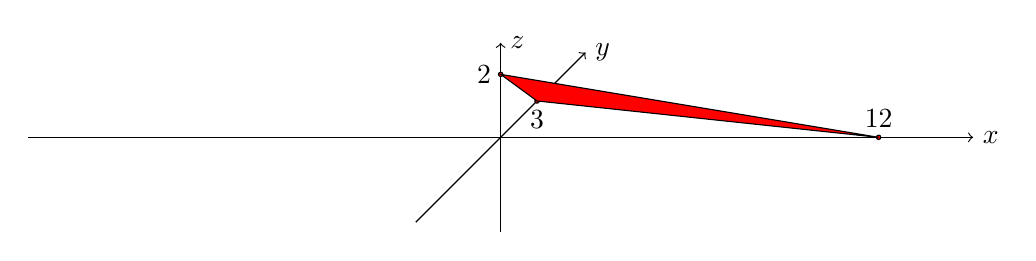
\begin{tikzpicture}[rotate around x=-90, scale=0.4]
      % Draw the first octant of a plane in 3D
      \draw[->] (-15,0,0) -- (15,0,0) node[right] {$x$};
      \draw[->] (0,-7,0) -- (0,7,0) node[right] {$y$};
      \draw[->] (0,0,-3) -- (0,0,3) node[right] {$z$};
      \draw[fill=red] (0,0,2) circle (2pt) node[left] {$2$};
      \draw[fill=red] (12,0,0) circle (2pt) node[above] {$12$};
      \draw[fill=red] (0,3,0) circle (2pt) node[below] {$3$};
      \draw[fill=red] (0,0,2) -- (12,0,0) -- (0,3,0) -- cycle;
    \end{tikzpicture}
  \end{center}
  With these axis conventions it's a bit easier to see the plane:
  \begin{center}
    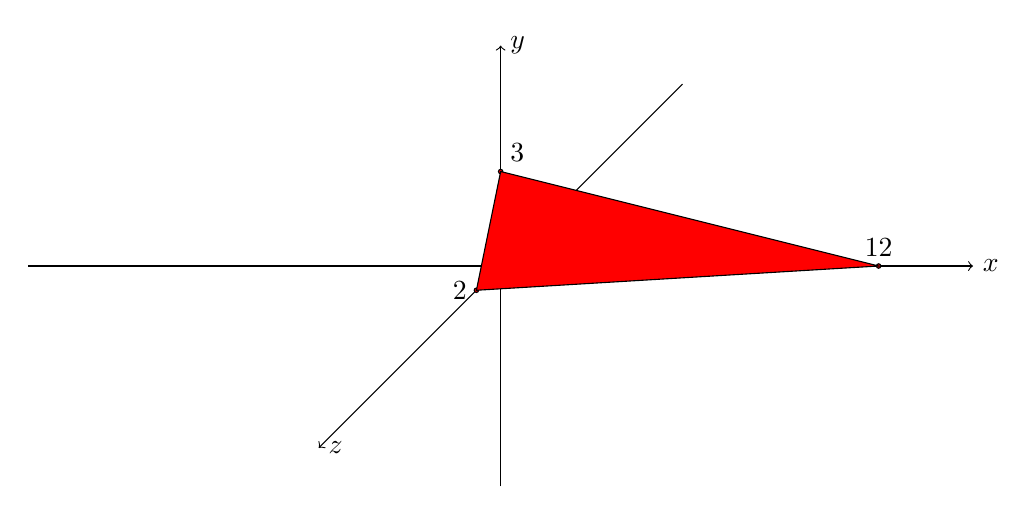
\begin{tikzpicture}[scale=0.4]
      % Draw the first octant of a plane in 3D
      \draw[->] (-15,0,0) -- (15,0,0) node[right] {$x$};
      \draw[->] (0,-7,0) -- (0,7,0) node[right] {$y$};
      \draw[->] (0,0,-15) -- (0,0,15) node[right] {$z$};
      \draw[fill=red] (0,0,2) circle (2pt) node[left] {$2$};
      \draw[fill=red] (12,0,0) circle (2pt) node[above] {$12$};
      \draw[fill=red] (0,3,0) circle (2pt) node[above right] {$3$};
      \draw[fill=red] (0,0,2) -- (12,0,0) -- (0,3,0) -- cycle;
    \end{tikzpicture}
  \end{center}
\end{pracsol}

\subsection*{10.1. Vector-valued functions---limits, derivatives, and continuity}
\begin{practice}p.802 \#14\end{practice}
\begin{pracsol}
  The $\bj$-component of $\br(t)$ is continuous at $t=1$, so the $\bj$-component of the limit will be $\frac{1+1}{1^2+1}=\frac 22=1$.

  The $\bi$-component is not continuous, but standard calculus limit techniques yield that
  \[\lim_{t\to 1}\frac{t-1}{t^2-1}=\lim_{t\to 1}\frac{1}{t+1}=\frac 12,\]
  so finally
  \[\lim_{t\to 1}\br(t)=\frac12\bi+\bj.\]
\end{pracsol}
\begin{practice}p.802 \#23\end{practice}
\begin{pracsol}
  According to Theorem 5,
  \[\br'(t)=-e^{-t}\bi-\frac{2t+4t^3}{t^2+t^4}\bj=-e^{-t}\bi-\frac{2+4t^2}{t+t^3}\bj.\]
  Therefore,
  \[\br''(t)=e^{-t}\bi-\frac{4t^4+2t^2+2}{(t+t^3)^2}\bj.\]
\end{pracsol}
\begin{practice}p.802 \#54\end{practice}
\begin{pracsol}
  We calculate the limit component-wise. The $\bi$-component is the classic sandwich theorem limit $\lim_{t\to 0}\frac{\sin(t)}t=1$. The $\bj$-component involves a function which is continuous at $t=0$, so the limit there is $\frac{0}{\cos(0)}=0$. The $\bk$-component can be written as
  \[\lim_{t\to 0}\frac{\sin(t)}{\cos(t)t}=\lim_{t\to 0}\frac 1{\cos(t)}\lim_{t\to 0}\frac{\sin(t)}{t}=1\cdot 1=1.\]
  All in all, the desired limit is equal to $\bi+\bk$.
\end{pracsol}

\subsection*{10.2. Velocity and acceleration}
\begin{practice}p.812 \#2\end{practice}
\begin{pracsol}
  The velocity is
  \[\bv(t)=\br'(t)=-2t\bi-20t^3\bk.\]
  The speed is
  \[v(t)=\|\bv(t)\|=\sqrt{(-2t)^2+(-20t^3)^2}=\sqrt{4t^2+400t^6}=2\sqrt{t^2+100t^6}.\]
  The acceleration is
  \[\ba(t)=\bv'(t)=-2\bi-60t^2\bk.\]
\end{pracsol}
\begin{practice}p.812 \#7\end{practice}
\begin{pracsol}
  \begin{align*}
    \bv(t) &= 2t\sin(t^2)\bi+2t\cos(t^2)\bj+3t^2\bk\\
    v(t) &= \|\bv(t)\|=\sqrt{4t^2+9t^4}\\
    \ba(t) &= (4t^2\cos(t^2)+2\sin(t^2))\bi-(4t^2\sin(t^2)-2\cos(t^2))\bj+6t\bk.
  \end{align*}
\end{pracsol}
\begin{practice}p.812 \#9\end{practice}
\begin{pracsol}
  Since the acceleration is $\ba(t)=-32\bk$, velocity is $\bv(t)=-32t\bk+\bv_0$ and position is $\br(t)=-16t^2\bk+t\bv_0+\br_0$. Finally, $\br(t)=-16t^2\bk+t(3\bi-2\bj+\bi)+2\bi-5\bk=(3t+2)\bi-2t\bj-(16t^2-t+5)\bk$.
\end{pracsol}
\begin{practice}p.812 \#34\end{practice}
\begin{pracsol}
  We set our coordinates so that everything is happening in the $xz$-plane, with the ball being thrown to the right (so the $\bi$-component of the velocity is positive at all times). Also let us say that the cliff is at $(0,0,500)=500\bk$, so this is the rock's initial position $\br_0$ as well.

  The initial velocity of the ball is
  \[\bv_0=50\cos\frac{\pi}6\bi+50\sin\frac{\pi}6\bj=25\sqrt3\bi+25\bk.\]
  Using the formula from the previous practice problem, we obtain
  \[\begin{split}
    \br(t) &= -16t^2\bk+t\bv_0+\br_0\\
    &= -16t^2\bk+25t\sqrt3 t\bi+25t\bk+500\bk\\
    &= 25\sqrt3 t\bi + (-16t^2+25t+500)\bk.
  \end{split}\]
  The rock hits the ground at the time $t$ when the $\bk$-component of $\br(t)$ is zero, in other words, at the positive solution to the quadratic equation $-16t^2+25t+500=0$. The solution is $t=\frac5{32}(5+3\sqrt{145})\approx 6.43$ seconds. At this value of $t$, the rock has traveled
  \[25\sqrt3 \cdot \frac5{32}(5+3\sqrt{145})\approx 278.24\text{ feet}.\]
\end{pracsol}

\newpage

\section{Homework problems -- submit these}

\begin{problem}
  \leavevmode\begin{enumerate}[(a)]
    \item Give two examples of points that are on the line $\ell\colon x=-3t+4,y=-t+6,z=t+4$. Prove that your examples work.
    \begin{solution}
      For the first point, we can pick $t=0$: then $x=4,y=6,z=4$, so the correspoinding point is $(4,6,4)$.

      For the second point let's set $t=1$: then $x=1,y=5,z=5$, so the correspoinding point is $(1,5,5)$.

      The proof that the examples work is completely contained in the above work, because a point $P$ is on the line $\ell$ given by $\br(t)$ if and only if there exists $t$ such that $\br(t)=P$.
    \end{solution}
    \item Show that the line $\ell$ (from part (a)) is contained inside the plane $V\colon 3x-7y+2z=-22$.
    \begin{solution}
      We have $\ell\subseteq V$ iff for every point $P$ in $\ell$, $P$ is also in $V$.

      We have $P$ is in $V$ for every $P$ in $\ell$ iff for every $t\in\bR$, the point $(-3t+4,-t+6,t+4)$ is in $V$.

      We have that $(-3t+4,-t+6,t+4)$ is in $V$ for every $t\in\bR$ iff for every $t\in\bR$, $3(-3t+4)-7(-t+6)+2(t+4)=-22$.

      So we must check that this equation is an identity, in other words holds for all $t$. Let's evaluate the left hand side:
      \[3(-3t+4)-7(-t+6)+2(t+4)=-9t+12+7t-42+2t+8=0t-22=-22,\]
      so indeed the equation $3(-3t+4)-7(-t+6)+2(t+4)=-22$ holds for all $t$.
    \end{solution}
    \item There should be a line which is contained in the same plane $V$ and perpendicular to $\ell$. Find a parametrization for it.
    \begin{solution}
      It takes a bit of thinking to come up with an idea, but the most obvious idea is that the direction vector for the desired line must be perpendicular to both $\ell$ and the normal $\bn$ to $V$, which implies that the desired direction vector must be parallel to $\mathbf m_\ell\times\bn$, where $\mathbf m_\ell$ is the direction vector for $\ell$.

      We have $\mathbf m_\ell=(-3,-1,1)$ because these are the coefficients of $t$ in the equations for $\ell$. We have $\bn=(3,-7,2)$ because these are the coefficients of $x,y,z$ respectively in the equation for $V$. So we can take our desired direction vector $\mathbf m$ to be
      \[\mathbf m_\ell\times\bn=(-3,-1,1)\times(3,-7,2)=(-2-(-7),3-(-6),21-(-3))=(5,9,24).\]
      We can pick any point in the plane $V$ as the starting point of the new line. Fortunately, we can pick $(4,6,4)$ from part (a), since we know it is on $\ell$, and so is in $V$ by part (b).

      So our parametrization can be
      \[\br(t)=(4,6,4)+t(5,9,24).\]
      (Note: Any direction vector parallel to $(5,9,24)$, including $(-5,-9,-24)$ is valid as well.)

      Catherine May wrote up a nice solution including a very nice illustration. I've included it below:
      \begin{center}
        \includegraphics[width=\textwidth]{nice/p2.1c_catherine.png}
        \includegraphics[width=\textwidth]{nice/p2.1c_catherine_page_2.png}
      \end{center}
    \end{solution}
    \item Is the line satisfying the conditions of part (c) unique? Give a brief explanation.
    \begin{solution}
      No, any other point on $\ell$ (or indeed, in $V$) can be used as the starting point of the line. For example, we could have taken $(1,5,5)$ instead and obtained
      \[\br(t)=(1,5,5)+t(5,9,24).\]
    \end{solution}
  \end{enumerate}
\end{problem}

\begin{problem}
  For parts (a) and (b), sketch the trajectory of the following vector-valued functions as $t$ ranges over the real numbers (except at points where the function is undefined).
  \begin{enumerate}[(a)]
    \item $\br(t)=t\cos(t)\bi+t\sin(t)\bj+t\bk$.
    \begin{solution}
      \begin{center}
        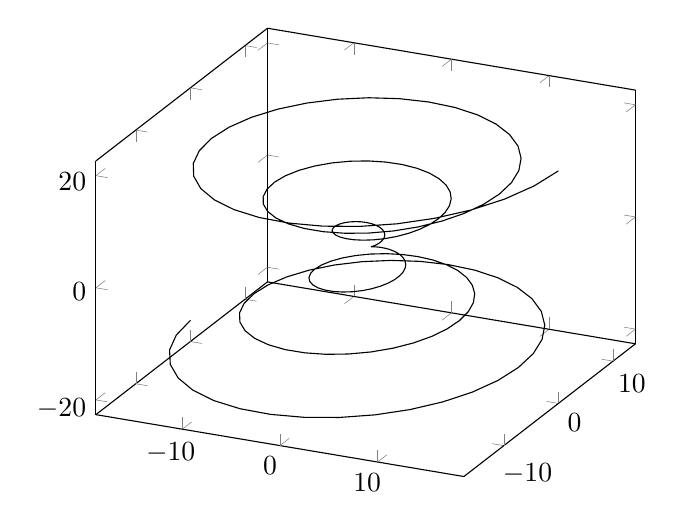
\begin{tikzpicture}
          \begin{axis}
          \addplot3[variable=t,domain=-6*pi:6*pi,samples=200,samples y=1] ({t*cos(deg(t))},{t*sin(deg(t))},t);
          \end{axis}
        \end{tikzpicture}
      \end{center}
    \end{solution}
    \item $\br(t)=(\frac 1{1-t},\frac{2-t}{1-t},\frac{3-2t}{1-t})$.
    \begin{solution}
      \begin{center}
        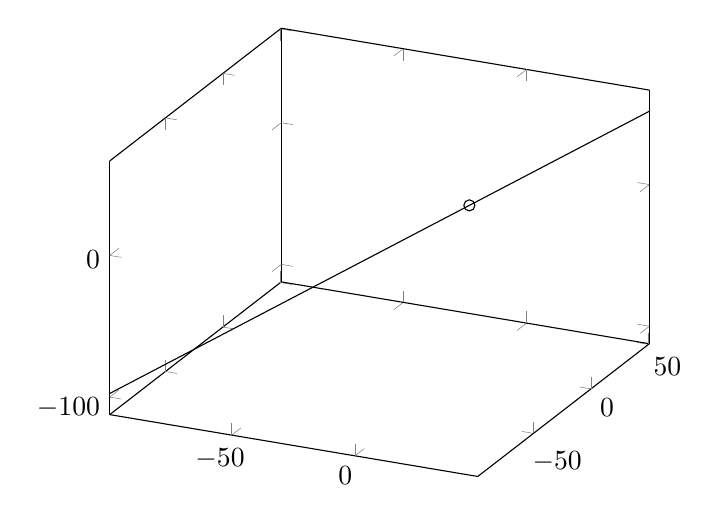
\begin{tikzpicture}
          \begin{axis}
          \addplot3[variable=t,domain=-3:3,samples=200,samples y=1] ({1/(1-t)}, {(2-t)/(1-t)}, {(3-2*t)/(1-t)});
          \draw (0,1,2) circle (2pt);
          \end{axis}
        \end{tikzpicture}
      \end{center}
    \end{solution}
    \item Let $\br(t)$ be as in part (b). What is $\lim_{t\to \infty}\br(t)$? What is $\lim_{t\to 1}\br(t)$?
    \begin{solution}
      \begin{align*}
        \lim_{t\to\infty}\br(t) &= (0,1,2). \\
        \lim_{t\to 1}\br(t) &\text{ is undefined}.
      \end{align*}
    \end{solution}
    \item You may have found that the trajectory of $\br(t)$ in (b) is a line (without one point). Explain how it can be that the trajectory of $\br(t)$ is a line despite the fact that the component functions are not linear functions.
    \begin{solution}
      $\br(t)$ can be expressed as $\mathbf s(\phi(t))$ where $\mathbf s(t)=(t,t+1,t+2)$ and $\phi(t)=\frac{1}{1-t}$. Indeed,
      \[\begin{split}
        \br(t)&=\left(\frac 1{1-t},\frac{2-t}{1-t},\frac{3-2t}{1-t}\right)\\
        &= \left(\frac{1}{1-t},1+\frac{1}{1-t},2+\frac{1}{1-t}\right)\\
        &= (\phi(t),1+\phi(t),2+\phi(t))\\
        &= \mathbf s(\phi(t)).
      \end{split}\]

      This shows that $\br$ is a reparametrization of the linear vector-valued-function $\mathbf s$. This means that every point on the trajectory of $\br(t)$ is on the trajectory of $\mathbf s(t)$ (Not necessarily vice versa, though. For example, $\phi(t)$ never equals 0, so $\br(t)$ will never hit the point $(0,1,2)$. Hence the hole shown in part (b)). The trajectory of $\mathbf s(t)$ is a line.

      (Relevant page of textbook: p.817.)

      Warning: Some people said you can factor out $1/(1-t)$ and get a linear function in what remains. This is a \textbf{bogus} explanation. In fact, you can plot the example $t\mapsto (t^2,t^3,t^2)$ to see that it is a counterexample to the factoring explanation. The difference between the two explanations lies in the fact that multiplication is not the same as composition.

      Another really nice way to prove this that I saw in some students' submissions is to show that the velocity vector $\br'(t)$ points in the same direction for all $t$. In fact,
      \[\br'(t)=\left(\frac{1}{(1-t)^2},\frac{1}{(1-t)^2},\frac{1}{(1-t)^2}\right)\parallel(1,1,1)\text{ for all }t.\]
      Well done!
    \end{solution}
  \end{enumerate}
  \textbf{Note}: If you use \LaTeX, you can hand-draw the pictures, save them into the folder (e.g.\ for Overleaf, you can just upload the picture), then import the picture via \verb|\includegraphics|. (You may need to add the \texttt{graphicx} package to the preamble if the command isn't recognized.)
\end{problem}

\begin{problem}
  \leavevmode
  \begin{enumerate}[(a)]
    \item Let $\br(t)=(x(t),y(t),z(t))$ be a vector-valued function representing the position of a particle at time $t$. Show that the particle's speed is increasing exactly when
    \[\frac d{dt}(x'(t)^2+y'(t)^2+z'(t)^2)>0.\]
    \begin{solution}
      The particle's speed is increasing iff
      \begin{align*}
        \frac d{dt}\|\br'(t)\| &>0\\
        \iff\frac d{dt}\sqrt{x'(t)^2+y'(t)^2+z'(t)^2} &>0\\
        \xLeftrightarrow{\text{chain rule}}\frac{(x'(t)^2+y'(t)^2+z'(t)^2)'}{2\sqrt{x'(t)^2+y'(t)^2+z'(t)^2}} &>0\\
        \iff (x'(t)^2+y'(t)^2+z'(t)^2)'&>0,
      \end{align*}
      the last step following from the fact that $2\sqrt{x'(t)^2+y'(t)^2+z'(t)^2}$ is always non-negative.

      Another valid solution is to prove the general fact that $\frac d{dt}\sqrt{f(t)}>0$ iff $\frac d{dt}f(t)>0$ using the chain rule, shortcutting lines 2 and 3 in the above chain of logic.
    \end{solution}
    \item Using part (a), show that the speed of a moving particle is increasing if the angle between the velocity and acceleration vectors is always acute. Show that the speed of the particle is decreasing if the angle is always obtuse.
    \begin{solution}
      First, notice that the angle between two vectors $\bv,\bw$ is acute iff $0<\theta<\frac{\pi}2$ (where $\theta$ is the angle between $\bv$ and $\bw$), iff $\cos\theta>0$, iff $\bv\cdot\bw>0$ (by the cosine angle formula $\bv\cdot\bw=\|\bv\|\|\bw\|\cos\theta$).

      The two vectors concerned here are $\br'(t)$ and $\br''(t)$. Finally, the particle's speed is increasing iff (first step is by part (a))
      \begin{align*}
        (x'(t)^2+y'(t)^2+z'(t)^2)' &>0\\
        \iff 2x'(t)x''(t)+2y'(t)y''(t)+2z'(t)z''(t) &>0\\
        \iff 2(x'(t),y'(t),z'(t))\cdot(x''(t),y''(t),z''(t))&>0\\
        \iff 2\br'(t)\cdot\br''(t) &> 0\\
        \iff \br'(t)\cdot\br''(t) &> 0\\
        \iff\text{the angle between $\br'(t)$ and $\br''(t)$ }&\text{is acute}.
      \end{align*}
      Exactly the same logic but with $<$ instead of $>$ proves the statement for obtuse angles.

      Seth Brantzeg had a nice different solution using projections. It is shown below:
      \begin{center}
        \includegraphics[width=\textwidth]{nice/p2.3b_seth.png}
      \end{center}
    \end{solution}
  \end{enumerate}
\end{problem}

\begin{problem}
  Find a formula for the distance between the two planes with Cartesian equations $Ax+By+Cz=D_1$ and $Ax+By+Cz=D_2$. You can use the following fact: if $P$ and $Q$ are two points on the two respective planes with minimum possible distance, then the vector $\overrightarrow{PQ}$ is perpendicular to both planes.

  (This should be a puzzling problem at first. Practice your problem solving! See hint if you are stuck.)
\end{problem}
\begin{solution}
  Let $P=(x,y,z)$ and $Q$ be as in the hint: $P$ is on the first plane, $Q$ is on the second plane, and $Q$ is chosen so that $\|\overrightarrow{PQ}\|$ is minimal.

  According to the fact in the problem, $\overrightarrow{PQ}\parallel\bn$, where $\bn=(A,B,C)$ is the common normal vector to both planes. (The fact that $\bn=(A,B,C)$ is because those are the coefficients of $x,y,z$ in both planes.)

  So let $\overrightarrow{PQ}=\lambda\bn$. Moreover, we have the following:
  \begin{align*}
    P\cdot\bn&= D_1\\
    Q\cdot\bn &= D_2,
  \end{align*}
  because, for example, the expression $P\cdot\bn$ equals $(x,y,z)\cdot(A,B,C)=Ax+By+Cz$ which is exactly equal to $D_1$ because of the fact that $P$ lies on the first plane. Similar reasoning holds for $Q$. Therefore,
  \[\overrightarrow{PQ}\cdot\bn=(Q-P)\cdot \bn=Q\cdot \bn-P\cdot \bn=D_2-D_1,\]
  But $\overrightarrow{PQ}\cdot\bn=(\lambda\bn)\cdot\bn=\lambda\|\bn\|^2$. Therefore, $\lambda\|\bn\|^2=D_2-D_1$, so $\lambda=\frac{D_2-D_1}{\|\bn\|^2}$. Finally,
  \[\|\overrightarrow{PQ}\|=\|\lambda\bn\|=|\lambda|\|\bn\|=\frac{|D_2-D_1|}{\|\bn\|^2}\|\bn\|=\frac{|D_2-D_1|}{\sqrt{A^2+B^2+C^2}}.\]
\end{solution}

\begin{problem}
  How difficult was each problem? Rate each problem (and part) on a difficulty scale from 1 to 7, where 1 means ``super easy, barely an inconvenience!'' and 7 means ``hardest problem I've ever done.''
\end{problem}

\newpage

\section{Hints}
\begin{hint}[Hint for 1(a)]
  Remember that proof just means something like ``watertight logical argument for why the claim is true''; in particular, perhaps the work you have already proves that the examples work!
\end{hint}

\begin{hint}[Hint for 1(b)]
  Show that every point $(x,y,z)$ of the line satisfies the equation of the plane.
\end{hint}

\begin{hint}[Hint for 1(c)]
  Cross products are amazingly useful\ldots

  More specifically, remember that the cross product of two vectors gives a vector perpendicular to both of them.
\end{hint}

\begin{hint}[Hint for 2(a) and 2(b)]
  I did not have another method in mind apart from making a table of values and connecting the dots.
\end{hint}

\begin{hint}[Hint for 2(d)]
  The following may be a useful idea: If $g\colon\bR\to\bR$ is a real-valued function and $\br(t)$ has a certain trajectory, then $\br(g(t))$ will follow the same trajectory, just traversed differently (according to $g$).

  In other words, reparametrization.

  There is also an important algebra manipulation that needs to be done to the expression for $\br(t)$ to make the idea visible. Check out problem 1(a) in this week's discussion for an example.
\end{hint}

\begin{hint}[Hint for 3]
  A common tactic in calculus to avoid the painful process of computing derivatives of square roots of a function is to observe that the derivative of the square root of a function is positive iff the derivative of the function itself is positive. (You can prove this using the chain rule.)
\end{hint}

\begin{hint}[Hint for 4]\leavevmode
  \begin{itemize}
    \item Write $P=(x,y,z)$ to denote an arbitrary point on the first plane. Let $Q$ be the point on the other plane with minimial distance to $P$.
    \item According to the fact in the problem, $\overrightarrow{PQ} \parallel \bn$, where $\bn$ is the common normal vector to both planes.
    \item Therefore, $\overrightarrow{PQ}=\lambda\bn$ for some $\lambda\in\bR$. This is the most important observation to make.
    \item The second most important observations: What is $P\cdot\bn$? What is $Q\cdot\bn$? (The dot product of a point with a vector is calculated in the same way as the dot product of two vectors.)
    \item To check yourself, the answer is
    \[\frac{|D_2-D_1|}{\sqrt{A^2+B^2+C^2}}.\]
  \end{itemize}
\end{hint}
